\documentclass[letterpaper]{article}
\usepackage{flairs}%aaai
\usepackage{times}
\usepackage{helvet}
\usepackage{courier}
\usepackage{graphicx}
\usepackage{setspace}
\frenchspacing
\setlength{\pdfpagewidth}{8.5in}
\setlength{\pdfpageheight}{11in}
\pdfinfo{
/Title (Representation, Verification, and Visualization of Tarskian Interpretations for Typed First-order Logic)
/Author (Geoff Sutcliffe, Alexander Steen, Pascal Fontaine, Jack McKeown)}
\setcounter{secnumdepth}{2}  
\newcommand{\smalltt}[1]{\small \texttt{#1}}
\newenvironment{packed_itemize}{
\vspace*{-0.5em}
\begin{itemize}
\setlength{\partopsep}{0pt}
\setlength{\itemsep}{1pt}
\setlength{\parskip}{0pt}
\setlength{\parsep}{0pt}
}{\end{itemize}}
\renewcommand{\textfraction}{0.07}
\renewcommand{\topfraction}{0.9}

\begin{document}
% This file is an adoption of the style file for AAAI Press 
% proceedings, working notes, and technical reports.  This file is made 
% with minimal changes by explicit permission from AAAI.

\title{Representation, Verification, and Visualization of\\
Tarskian Interpretations for Typed First-order Logic}
\author{Anon One\\
Some where\\
Some place\\
Some country\\
\And
Anon Two\\
Some where\\
Some place\\
Some country\\
\And
Anon Three\\
Some where\\
Some place\\
Some country\\
\And
Anon Four\\
Some where\\
Some place\\
Some country}

\maketitle
\begin{abstract}
\begin{quote}
\end{quote}
\end{abstract}
%--------------------------------------------------------------------------------------------------
\section{Introduction}
\label{Introduction}

Automated Reasoning (AR), and Automated Theorem Proving (ATP) in particular, has largely focused
on the task of proving theorems from axioms - the derivation of conclusions that follow inevitably 
from known facts \cite{RV01-HAR}.
The axioms and conjecture to be proved (and hence become a theorem) are written in an 
appropriately expressive logic, and the proofs that are found are often similarly written in
logic \cite{SS+06}.
In this work we consider typed first-order logic in the form of \cite{Wal83,Sch85,Coh87},
%  higher-order \cite{And86}, and some 
% on-classical \cite{Pri08} logics, 
whose expressive power is sufficient for a wide range of topics \cite{Sut17}.
(This work is also applicable to untyped first-order logic where terms have the type $\iota$ 
and formulae have the type $o$, and can also be generalized to higher-order logics.)

In the last two decades the converse task of disproving conjectures, i.e., proving that a 
conjecture is not a theorem of the axioms, has become increasingly important.
This process depends on finding an {\em interpretation} of the formulae, i.e., a structure that
maps expressions written in the language of the formulae to domain elements and truth values.
In most cases the interpretation is a {\em model} of certain formulae, i.e., it maps those
formulae to {\em true}.
A disproof of a conjecture is a countermodel that provides an interpretation of the formulae 
that is a model of the axioms, but maps the conjecture to {\em false}.
A salient application area that harnesses this form of ATP is verification \cite{DKW08},
where a countermodel is used to pinpoint the reason why a proof obligation fails, and
correspondingly points to the location of the fault in the system being verified.
Other applications of model finding include checking the consistency of an axiomatization 
\cite{SS+17}, and finding a solution to a problem that is coded as a model finding problem 
\cite{Win82}.
This work describes a (new) format for representing interpretations using a TPTP language -
Sections~\ref{TPTP}~and~\ref{Interpretations}.

In addition to ATP systems that produce interpretations (typically models),
% proofs, e.g., Vampire \cite{KV13}, Leo-III \cite{SB18},
% % nanoCop-M \cite{Ott21}, 
% and ATP systems that find 
e.g., Paradox \cite{CS03}, FM-Darwin \cite{BF+09}, Nipick \cite{BN10-ITP},
there is a need for tools that support examination and use of the interpretations.
This paper examines the tasks of verifying models and visualizing interpretations, and describes 
new tools for these tasks - Sections~\ref{Verification}~and~\ref{Visualization}.

PF2ALL: application of visualization: understand the essence of a model, pedagogy in logic courses and formal methods.

\paragraph{Related Work:}
In \cite{SS+06} a TPTP format for interpretations with finite domains was defined, and has been 
adopted by some ATP systems that find finite models, e.g., Paradox and Vampire.
The SMT-LIB format \cite{BFT17} provides facilities to inspect or output models.  
SAT solvers generally output models as specified by the SAT competitions, in a simple format 
similar to the DIMACS input format.
Ad hoc formats are used by model finding systems, e.g., TO BE FILLED IN BY ALL.
+++
Nikolaj says ...
Z3 It produces models that define functions by expressions. For example a model of succ is 
Succ(x) =X+ 1
Works when domain is integer. Currently z3 does not implement infinite models for uninterpreted sorts. I would probably support infinite sorts by creating injection into an algebraic datatype and then support models that can be expressed over ADT.
See also https://microsoft.github.io/z3guide/docs/logic/Quantifiers
+++
Related work on verification and visualization of interpretations is sparse:
Model verification related work by Giles? Other?
% Pascal - know any from SMT? PF: no, to my best knowledge, and after a quick check on Google.
Visualization.
No related work. Alex - know any (other than your student)?

% This paper is organized as follows:
% Section~\ref{TPTP} introduces the TPTP World which provides the framework and languages used
% in this research.
% Section~\ref{Interpretations} discusses the nature of interpretations, and describes the new 
% representation of interpretations using a TPTP language.
% Section~\ref{Verification} provides the theory for verifying models, and describes the
% implementation of that theory in a model verification tool.
% Section~\ref{Visualization} introduces a novel way of visualizing interpretations, and
% proposes a tool for automating the visualization of interpretations written in the TPTP language.
% Section~\ref{Conclusion} concludes and discusses plans for future work.

%--------------------------------------------------------------------------------------------------
\section{The TPTP World and Languages}
\label{TPTP}

The TPTP World \cite{Sut17} is a well established infrastructure that supports research, 
development, and deployment of Automated Theorem Proving (ATP) systems.
The TPTP World includes the TPTP problem library,
% \cite{Sut09}, 
the TSTP solution library,
% \cite{Sut10}, 
standards for writing ATP problems and reporting ATP solutions,
% \cite{SS+06,Sut08-KEAPPA}, 
tools and services for processing ATP problems and solutions,
% \cite{Sut10}, 
and it supports the CADE ATP System Competition (CASC).
% \cite{Sut16}.
Various parts of the TPTP World have been deployed in a range of applications,
in both academia and industry.
% Since the first release of the TPTP problem library in 1993, many researchers have used the 
% TPTP World as an appropriate and convenient basis for ATP system research and development. 
% Over the years the TPTP World has provided a platform upon which ATP users have presented their 
% needs to ATP system developers, who have then adapted their ATP systems to the users’ needs.
The web page {\smalltt{https://www.tptp.org}} provides access to all components.

The TPTP languages \cite{Sut22-IGPL} are one of the keys to the success of the TPTP World.
The languages are used for writing both TPTP problems and TSTP solutions, which enables convenient 
communication between different systems and researchers. 
It also enables tool exchange, tool integration, and comparable experimental results.
Originally the TPTP World supported only first-order clause normal form (CNF).
% \cite{SS98-JAR}.
Over the years full first-order form (FOF),
% \cite{Sut09}, 
typed first-order form (TFF).
% \cite{SS+12,BP13-TFF1}, 
typed extended first-order form (TXF),
% \cite{SK18}, 
typed higher-order form (THF),
% \cite{SB10,KSR16}, 
and non-classical forms (NTF),
% \footnote{%
% There are many ``non-classical logics'', including multi-valued logics \cite{Aug17},
% paraconsistent logics \cite{Pri02}, relevance logics \cite{AB75}, etc.
% In this work we are interested in those that admit Kripke interpretation \cite{Kri63},
% e.g., modal logics \cite{BBW06}.}
% \cite{SF+22} 
have been added.
% A general principle of the TPTP language is ``we provide the syntax, you provide the semantics''.
% As such, there is no a priori commitment to any semantics for the languages, although in almost 
% all cases the intended logic and semantics are well known.
All the typed languages include constructs for arithmetic.
This work applies to all the languages; TF0 (the monomorphic form of TFF) \cite{SS+12} 
% and NX0 \cite{SF+22} forms are 
is used as the example.

The top level building blocks of the TPTP language are {\em annotated
formulae}.
An annotated formula has the form:\\
\hspace*{0.5cm}{\em language}{\tt (}{\em name}{\tt ,}
{\em role}{\tt ,}
{\em formula}{\tt ,}
{\em source}{\tt ,}
{\em useful\_info}{\tt ).}\\
The {\em language}s supported are clause normal form (\smalltt{cnf}), first-order form 
(\smalltt{fof}), typed first-order form (\smalltt{tff}), and typed higher-order form 
(\smalltt{thf}).
These are used by the corresponding languages, with TXF inheriting {\tt tff} and the non-classical 
languages their corresponding underlying languages.
The {\em role}, e.g., \smalltt{axiom}, \smalltt{lemma}, \smalltt{conjecture},
defines the use of the formula in an ATP system.
In the {\em formula}, terms and atoms follow Prolog conventions.
%  --
% functions and predicates start with a lowercase letter or are {\tt '}single quoted{\tt '}, and 
% variables start with an uppercase letter.
The TPTP language also supports interpreted symbols, which either start with a
{\tt \$}, or are composed of non-alphanumeric characters, e.g., the truth
constants \smalltt{\$true} and \smalltt{\$false}, and integer/rational/real
numbers such as 27, 43/92, -99.66.
The basic logical connectives are
{\tt !}, {\tt ?}, {\tt \verb|~|}, {\tt |}, {\tt \&}, {\tt =>}, {\tt <=},
{\tt <=>}, and {\tt <\verb|~|>},
for
$\forall$, $\exists$, $\neg$, $\vee$, $\wedge$, $\Rightarrow$, $\Leftarrow$,
$\Leftrightarrow$, and $\oplus$ respectively.
Equality and inequality are expressed as the infix operators {\tt =} and
{\tt !=}.
The {\em source} and {\em useful\_info} are optional.
Annotated formulae (using TF0, as described in Section~\ref{TF0}) can be seen in 
Figures~\ref{TF0FiniteProblem}-\ref{TF0InfiniteVerification}.

%--------------------------------------------------------------------------------------------------
\subsection{The TF0 Language}
\label{TF0}

% is a typed first-order language extended with FOOL logic constructs.
TF0 is a typed first-order language.
Every function and predicate symbol is declared before its use, with a type signature that 
specifies the types of the symbol’s arguments and result.
The TF0 types are
(i)~the predefined types \smalltt{\$i} for individuals and \smalltt{\$o} for booleans; 
(ii)~the predefined arithmetic types \smalltt{\$int}, \smalltt{\$rat}, and \smalltt{\$real}; 
(iii)~user-defined types that have been declared to be of the kind \smalltt{\$tType}.
TF0 type signatures are 
(i)~individual types;
(ii)~function types from non-boolean argument types to result types;
(iii)~predicate types from non-boolean argument types to boolean.
The equality predicates {\tt =} and {\tt !=} are ad hoc polymorphic over all types, and the types 
of arithmetic predicates and functions are ad hoc polymorphic over the arithmetic types.
% TX0 formulae are those of first-order logic, extended to allow boolean variables and terms.
% TX0 additionally supports tuples, conditional expressions, and let expressions, but they are
% not used in this paper (see \cite{SK18} for the details).
Figures~\ref{TF0FiniteProblem}~and~\ref{TF0InfiniteProblem} are examples of problems in TF0.  Their associated (counter)models are discussed in Section~\ref{Interpretations}.

\begin{figure}[htbp]
\scriptsize
\setstretch{0.8}
\begin{verbatim}
%--------------------------------------------------------
tff(man_type,type,           man: $tType ).
tff(grade_type,type,         grade: $tType ).
tff(john_decl,type,          john: man ).
tff(a_decl,type,             a: grade ).
tff(f_decl,type,             f: grade ).
tff(grade_of_decl,type,      grade_of: man > grade ).
tff(created_equal_decl,type, 
    created_equal: ( man * man ) > $o ).

tff(all_created_equal,axiom,
    ! [H1: man,H2: man] : created_equal(H1,H2) ).

tff(john_failed,axiom,
    grade_of(john) = f ).

tff(someone_got_an_a,axiom,
    ? [H: man] : grade_of(H) = a ).

tff(distinct_grades,axiom,
    a != f ).

tff(equality_lost,conjecture,
    ! [H1: man,H2: man] :
      ( created_equal(H1,H2)
    <=> ( H1 = H2 ) ) ).
%--------------------------------------------------------
\end{verbatim}
\caption{A TF0 problem (with a finite countermodel)\\
{\scriptsize {\tt https://raw.githubusercontent.com/GeoffsPapers/\\
ModelVerification/main/TFF\_Finite.p}}}
\label{TF0FiniteProblem}
\end{figure}

\begin{figure}[htbp]
\scriptsize
\setstretch{0.8}
\begin{verbatim}
%--------------------------------------------------------
tff(person_type,type,        person: $tType ).
tff(bob_decl,type,           bob: person ).
tff(child_of_decl,type,      child_of: person > person ).
tff(is_descendant_decl,type, 
    is_descendant: ( person * person ) > $o ).

tff(descendents_different,axiom,
    ! [A: person,D: person] : 
      ( is_descendant(A,D) => A != D ) ).

tff(descendent_transitive,axiom,
    ! [A: person,C: person,G: person] :
      ( ( is_descendant(A,C) & is_descendant(C,G) ) 
     => is_descendant(A,G) ) ).

tff(child_is_descendant,axiom,
    ! [P: person] : is_descendant(P,child_of(P)) ).

tff(all_have_child,axiom,
    ! [P: person] : ? [C: person] : C = child_of(P) ).
%--------------------------------------------------------
\end{verbatim}
\caption{A TF0 problem (with an infinite model)\\
{\scriptsize {\tt https://raw.githubusercontent.com/GeoffsPapers/\\
ModelVerification/main/TFF\_Infinite.p}}}
\label{TF0InfiniteProblem}
\end{figure}

%--------------------------------------------------------------------------------------------------
% \subsection{The NXF Language}
% \label{NXF}

%--------------------------------------------------------------------------------------------------
\section{Interpretations}
\label{Interpretations}

A Tarskian-style \cite{TV56} interpretation of formulae in a classical typed logic consists of 
non-empty domains (one for each type - just one domain in the case of untyped logic), and 
interpretations of the symbols (of the language induced by the formulae) with respect to the domains 
\cite{Hun96}.
An interpretation of given formulae can normally interpret all terms and formulae that can be 
written in the language induced by the given formulae, but in some circumstances an interpretation 
can interpret only (at least) the given formulae; such an interpretation is a {\em partial
interpretation}.

The domains of an interpretation may be finite or infinite.
Interpretations with only finite domains are called {\em finite interpretations}, and
interpretations with one of more infinite domains are called {\em infinite interpretations}.
Finite domains are commonly explicitly enumerated, but can also take other forms, e.g., the 
finite Herbrand Universe of a Herbrand interpretation \cite{Her30}.
Infinite domains can take several forms, including explicitly specified, e.g., the integers,
explicitly generated, e.g., closed terms representing Peano numbers, algebraic numbers (real
closed fields), and the infinite Herbrand Universe of a Herbrand interpretation.

It is noted that in addition to Tarskian-style interpretations that provide an explicit
interpretation of the symbols, a Herbrand model of clausal formulae can also be embodied in a 
saturation \cite{BG+01}, i.e., a fixed point for a set of clauses at which further application 
of a complete inference system does not generate any new clauses.
Indeed, this approach is adopted in saturation-based ATP systems such as E \cite{SCV19}, 
Prover9 \cite{McC-Prover9-URL}, Vampire, and Zipperposition \cite{VB+21}.
Unfortunately, a saturation tells you only that models exist, and very little about what they 
might look like. 
Saturations are difficult to interpret explicitly in a way that can be used constructively by 
users, and are thus a less useful form of interpretation.
This work considers the representation, verification, and visualization of only Tarskian-style 
interpretations with explicit symbol interpretation.

The notions of interpretations, models, partial interpretations, finite interpretations,
Herbrand interpretations, etc., are captured in the SZS ontologies \cite{Sut08-KEAPPA}, as
updated at \smalltt{https://www.tptp.org/cgi-bin/SeeTPTP? Category=Documents\&File=SZSOntology}

% A Kripke interpretation of a formulae in a non-classical logic consists of a set or worlds,
% an accessibility relation between those worlds, and a classical logic interpretation within each
% world \cite{}.
% The set of worlds may be finite or infinite.
 
%--------------------------------------------------------------------------------------------------
\subsection{Representing Interpretations in TF0}
\label{InterpretationsTF0}

As noted in Section~\ref{Introduction}, a TPTP format for interpretations with finite domains 
has previously been defined \cite{SS+06}, and has been adopted by some ATP systems.
Recently the need for a format for interpretations with infinite domains, and for a format for 
Kripke interpretations \cite{Kri63} of formulae written in the NTF language \cite{SF+22}, has 
led to the development of a new format for interpretations using the TPTP languages.
The changes allow for multiple interpretations to be given in a single file, which, in the case
of typed logics, share type declarations.
The underlying principle in unchanged: interpretations are represented using the same logic
as used by the formulae that are interpreted.
This provides the basis for verification of models, as explained in Section~\ref{Verification}.

The new format for an interpretation uses a single annotated formula with the role 
\smalltt{interpretation}, preceded by any necessary type declarations for typed logics.
The type declarations are those of the formulae being interpreted, and declarations for:
\begin{packed_itemize}
\item the types of the domains (unless already defined in the language, e.g., the type
      \smalltt{\$int});
\item the types of type-promotion functions that promote the types of the domains to the types 
      of the formulae; type-promotion is required to make the terms and formulae of the
      interpretation formula well-typed;
\item the types of the domain elements.
\end{packed_itemize}
\vspace*{-0.4em}
The \smalltt{interpretation} formula specifies 
\begin{packed_itemize}
\item the domain for each type in the formulae, including explicit or implicit specification
      of the distinct domain elements;
\item constraints making (in conjunction with the domain specifications) the type-promotion 
      functions into bijections;
\item interpretation of the formulae symbols.
\end{packed_itemize}

Figure~\ref{TF0FiniteInterpretation} is an interpretation with a finite domain - it is a 
countermodel for the problem in Figure~\ref{TF0FiniteProblem}.
The comments show which parts of the formula specify what aspects of the interpretation, per
the list above.
Note how:
\begin{packed_itemize}
\item the type-promotion functions are used to specify the domains;
\item the TPTP language's \smalltt{\$distinct} predicate makes the domain elements unequal to
      each other;
\item the domain specifications make the type-promotion functions surjective, which along
      with the constraint of injectivity makes the functions bijective;
\item functions applied to domain elements are interpreted by equating them to domain elements
      via appropriate type-promotion function, thus making the terms well-typed;
\item predicates applied to domain elements are interpreted directly by asserting them or their
      negation.
\end{packed_itemize}

\begin{figure}[htbp]
\scriptsize
\setstretch{0.8}
\begin{verbatim}
%--------------------------------------------------------
tff(man_type,type,           man: $tType ).
tff(grade_type,type,         grade: $tType ).
tff(john_decl,type,          john: man ).
tff(a_decl,type,             a: grade ).
tff(f_decl,type,             f: grade ).
tff(grade_of_decl,type,      grade_of: man > grade ).
tff(created_equal_decl,type, 
    created_equal: ( man * man ) > $o ).

%----Types of the domains
tff(d_man_type,type,         d_man: $tType).
tff(d_grade_type,type,       d_grade: $tType).
%----Types of the promotion functions
tff(d2man_decl,type,         d2man: d_man > man ).
tff(d2grade_decl,type,       d2grade: d_grade > grade ).
%----Types of the domain elements
tff(d_john_decl,type,        d_john: d_man ).
tff(d_gotA_decl,type,        d_gotA: d_man ).
tff(d_a_decl,type,           d_a: d_grade ).
tff(d_f_decl,type,           d_f: d_grade ).

tff(equality_lost,interpretation,
%----The domain for man is d_man
    ( ( ! [M: man] : ? [DM: d_man] : M = d2man(DM)
%----The d_man elements are d_john and d_gotA
      & ! [DM: d_man] : ( DM = d_john | DM = d_gotA )
      & $distinct(d_john,d_gotA)
%----The type promoter is a bijection
      & ! [DM1: d_man,DM2: d_man] :
          ( d2man(DM1) = d2man(DM2) => DM1 = DM2 )
%----The domain for grade is d_grade
      & ! [G: grade] : ? [DG: d_grade] : G = d2grade(DG)
%----The d_grade elements are d_a and d_f
      & ! [DG: d_grade]: ( DG = d_a | DG = d_f )
      & $distinct(d_a,d_f)
%----The type promoter is a bijection
      & ! [DG1: d_grade,DG2: d_grade] :
          ( d2grade(DG1) = d2grade(DG2) => DG1 = DG2 ) )
%----Interpret terms via the type-promoted domain
    & ( a = d2grade(d_a)
      & f = d2grade(d_f)
      & john = d2man(d_john)
      & grade_of(d2man(d_john)) = d2grade(d_f)
      & grade_of(d2man(d_gotA)) = d2grade(d_a) )
%----Interpret atoms as true of false
    & ( created_equal(d2man(d_john),d2man(d_john))
      & created_equal(d2man(d_john),d2man(d_gotA))
      & created_equal(d2man(d_gotA),d2man(d_john))
      & created_equal(d2man(d_gotA),d2man(d_gotA)) ) 
    ) ).
%----If John was not equal to the person who got an A:
%---- & ~ created_equal(d2man(d_john),d2man(d_gotA))
%---- & ~ created_equal(d2man(d_gotA),d2man(d_john))
%--------------------------------------------------------
\end{verbatim}
\caption{A TF0 interpretation with a finite domain \\
{\scriptsize {\tt https://raw.githubusercontent.com/GeoffsPapers/\\
ModelVerification/main/TFF\_Finite.s}}}
\label{TF0FiniteInterpretation}
\end{figure}

Figure~\ref{TF0InfiniteInterpretation} is an interpretation with an infinite domain - it is a model 
for the problem in Figure~\ref{TF0InfiniteProblem}.
The components are very much the same as for Figure~\ref{TF0FiniteInterpretation}, noting how:
\begin{packed_itemize}
\item the domain declaration uses the defined arithmetic type \smalltt{\$int};
\item there is no specification of the types of the domain elements or their inequality because 
      the type is defined;
\item universal quantification is used to specify the interpretation of functions and predicates
      for an infinite number of domain element argument tuples;
\item the interpretations of functions and predicates is not specified for argument tuples with 
      negative integer arguments - this is an example of a partial interpretation.
\end{packed_itemize}

\begin{figure}[htbp]
\scriptsize
\setstretch{0.8}
\begin{verbatim}
%--------------------------------------------------------
tff(person_type,type,        person: $tType ).
tff(bob_decl,type,           bob: person ).
tff(child_of_decl,type,      child_of: person > person ).
tff(is_descendant_decl,type, 
    is_descendant: ( person * person ) > $o ).

tff(int2person_decl,type,    int2person: $int > person ).

tff(people,interpretation,
%----Domain for type person is the integers
    ( ! [P: person] : ? [I: $int] : int2person(I) = P
%----The type promoter is a bijection
    & ! [I1: $int,I2: $int] : 
        ( int2person(I1) = int2person(I2) 
       => I1 = I2 )
%----Mapping people to integers. 
    & bob = int2person(0)
    & ! [I: $int] : 
        child_of(int2person(I)) = int2person($sum(I,1))
%----Interpretation of descendancy
    & ! [A: $int,D: $int] : 
        ( is_descendant(int2person(A),int2person(D)) 
      <=> $less(A,D) ) ) ).
%--------------------------------------------------------
\end{verbatim}
\caption{A TF0 interpretation with an infinite domain\\
{\scriptsize {\tt https://raw.githubusercontent.com/GeoffsPapers/\\
ModelVerification/main/TFF\_Infinite.s}}}
\label{TF0InfiniteInterpretation}
\end{figure}

%--------------------------------------------------------------------------------------------------
% \subsection{Kripke Interpretations}
% \label{Kripke}

%--------------------------------------------------------------------------------------------------
\section{Model Verification}
\label{Verification}

One way to verifying proofs output by ATP systems is to verify that each inference of the
implemented calculus is performed correctly; if the calculus is sound then the proof is
sound.
Inferences of logical consequence can be checked by forming a proof obligation whose axioms
are the parents of the inference and whose conjecture is the conclusion of the inference,
then discharging the obligation using a trusted ATP system. 
This ``semantic'' approach is taken in, e.g., SPASS \cite{WF+09} and in GDV \cite{Sut06}.
The same approach can be taken to verify that an interpretation is a model of given formulae, 
by proving each of the given formulae is a logical consequence of the interpretation formula.
The interpretation formula is supplied as an axiom, and each of the given formulae is proven
as a conjecture (or their conjunction can be proven).
The soundness of this approach relies on the fact that if a given formula is a logical consequence 
of the interpretation formula, then the given formula is interpreted as {\em true} by the model 
represented by the interpretation formula.

Proof

Implementation.
Problem's axioms and negated conjecture as conjectures (TPTP standard says can do separately,
but ATP systems take them as a disjunction to make them into one big conjunction - that's
harder to verify of course).

Figure~\ref{TF0InfiniteVerification} is the verification problem for the problem in 
Figure~\ref{TF0InfiniteProblem} and its model in Figure~\ref{TF0InfiniteInterpretation}.

\begin{figure}[htbp]
\scriptsize
\setstretch{0.8}
\begin{verbatim}
%--------------------------------------------------------
tff(person_type,type,        person: $tType ).
tff(bob_decl,type,           bob: person ).
tff(child_of_decl,type,      child_of: person > person ).
tff(is_descendant_decl,type, 
    is_descendant: ( person * person ) > $o ).

tff(int2person_decl,type,    int2person: $int > person ).

tff(people,axiom,
    ( ( ! [P: person] : ? [I: $int] : int2person(I) = P
      & ! [I1: $int,I2: $int] : 
          ( int2person(I1) = int2person(I2) 
         => I1 = I2 ) )
    & bob = int2person(0)
    & ! [I: $int] : 
        child_of(int2person(I)) = int2person($sum(I,1))
    & ! [A: $int,D: $int] : 
        ( is_descendant(int2person(A),int2person(D)) 
      <=> $less(A,D) ) ) ).

tff(prove_formulae,conjecture,
    ( ! [A: person,D: person] : 
        ( is_descendant(A,D) => A != D )
    & ! [A: person,C: person,G: person] :
        ( ( is_descendant(A,C) & is_descendant(C,G) )
       => is_descendant(A,G) )
    & ! [P: person] : is_descendant(P,child_of(P))
    & ! [P: person] : ? [C: person] : C = child_of(P) 
    ) ).
%--------------------------------------------------------
\end{verbatim}
\caption{The TF0 verification problem for 
Figures~\ref{TF0InfiniteProblem}~and~\ref{TF0InfiniteInterpretation}\\
{\scriptsize {\tt https://raw.githubusercontent.com/GeoffsPapers/\\
ModelVerification/main/TFF\_Infinite.s.p}}}
\label{TF0InfiniteVerification}
\end{figure}

%--------------------------------------------------------------------------------------------------
\section{Interpretation Visualization}
\label{Visualization}

Proof visualization is well-established, with several tools available, e.g., 
JACK TO INVESTIGATE.
Treehehe {\smalltt{https://chelsea.lol/Resources/COMP5209\_BattellC\_report.pdf}},
Evonne {\smalltt{https://lat.inf.tu-dresden.de/research/papers/2022/ALBABODAKOME-IJCAR22.pdf}},
ProofTree,
Anything from Dedukti?,
IDV \cite{TPS07}.
However, interpretation visualization has (to the knowledge of the authors) not been investigated.
JACK TO INVESTIGATE.
A way of visualizing finite interpretations for TFO formulae has been designed in this work, and 
a prototype implementation is available online as the IIV tool in the SystemOnTSTP 
\cite{Sut07-CSR} web interface {\smalltt{https://www.tptp.org/cgi-bin/SystemOnTSTP}}.

Figure~\ref{TF0FiniteIIV} is the visualization of the finite countermodel in 
Figure~\ref{TF0FiniteInterpretation}, with {\smalltt{john}} not created equal to the person
who got an {\smalltt{A}}.
The top row of inverted triangles are the types used in the given formulae,
while the bottom row of inverted triangles are the types of the domains in the interpretation
formula.
The row of inverted houses are the function and predicate symbols in the given formulae,
and the successive rows of ovals are the successive arguments for the symbols as used in the
specification of their interpretation.
Finally, the row of houses and boxes are the interpretations of the symbols applied to those
arguments; houses for functions and boxes for predicates.
For example, in the given formulae the type of {\smalltt{grade\_of}} is {\smalltt{grade}},
and {\smalltt{grade\_of(d\_john)}} is interpreted as {\smalltt{d\_f}}, which is of type
{\smalltt{d\_grade}} in the interpretation formula.

IIV provides some interactive features: Figure~\ref{TF0FiniteIIV} shows the situation with 
the cursor hovering over the lower {\smalltt{d\_john}} node on the path from 
{\smalltt{created\_equal}} to {\smalltt{\$true}}.
The nodes above are increasingly darker red (grey if printed) up to the type node {\smalltt{\$o}} 
that is the result type of {\smalltt{created\_equal}}, and of increasingly darker blue down to 
the type node {\smalltt{\$o}} that is the type of {\smalltt{\$true}}.
This interactive highlighting allows a user to quickly identify the interpretations for symbols
of the language by hovering over the inverted house nodes, to quickly find what symbols applied to
what domain elements are interpreted as which domain elements and boolean values by hovering over
the house and box nodes, and to quickly see how different domain elements affect the interpretation
of difference symbols by hovering over the oval nodes.
Here the cursor is hovering over a {\smalltt{d\_john}} node, showing how
{\smalltt{created\_equal(d\_john,d\_john)}} is interpreted as {\smalltt{\$true}}.
Details of the annotated formulae used to represent each node in the input to IIV are available 
in the ``Node Information'' box (which is to the left in reality, placed below here).
This interactive visualization is available in the IIV tool in SystemOnTSTP, using 
{\scriptsize {\tt https://raw.githubusercontent.com/ GeoffsPapers/ModelVerification/main/TFF\_Finite.s.IDV}}
as the ``URL to fetch from'', selecting {\tt IIV 0.0} as the ``System'', and clicking the
``Process Solution'' button.

\begin{figure}[htbp]
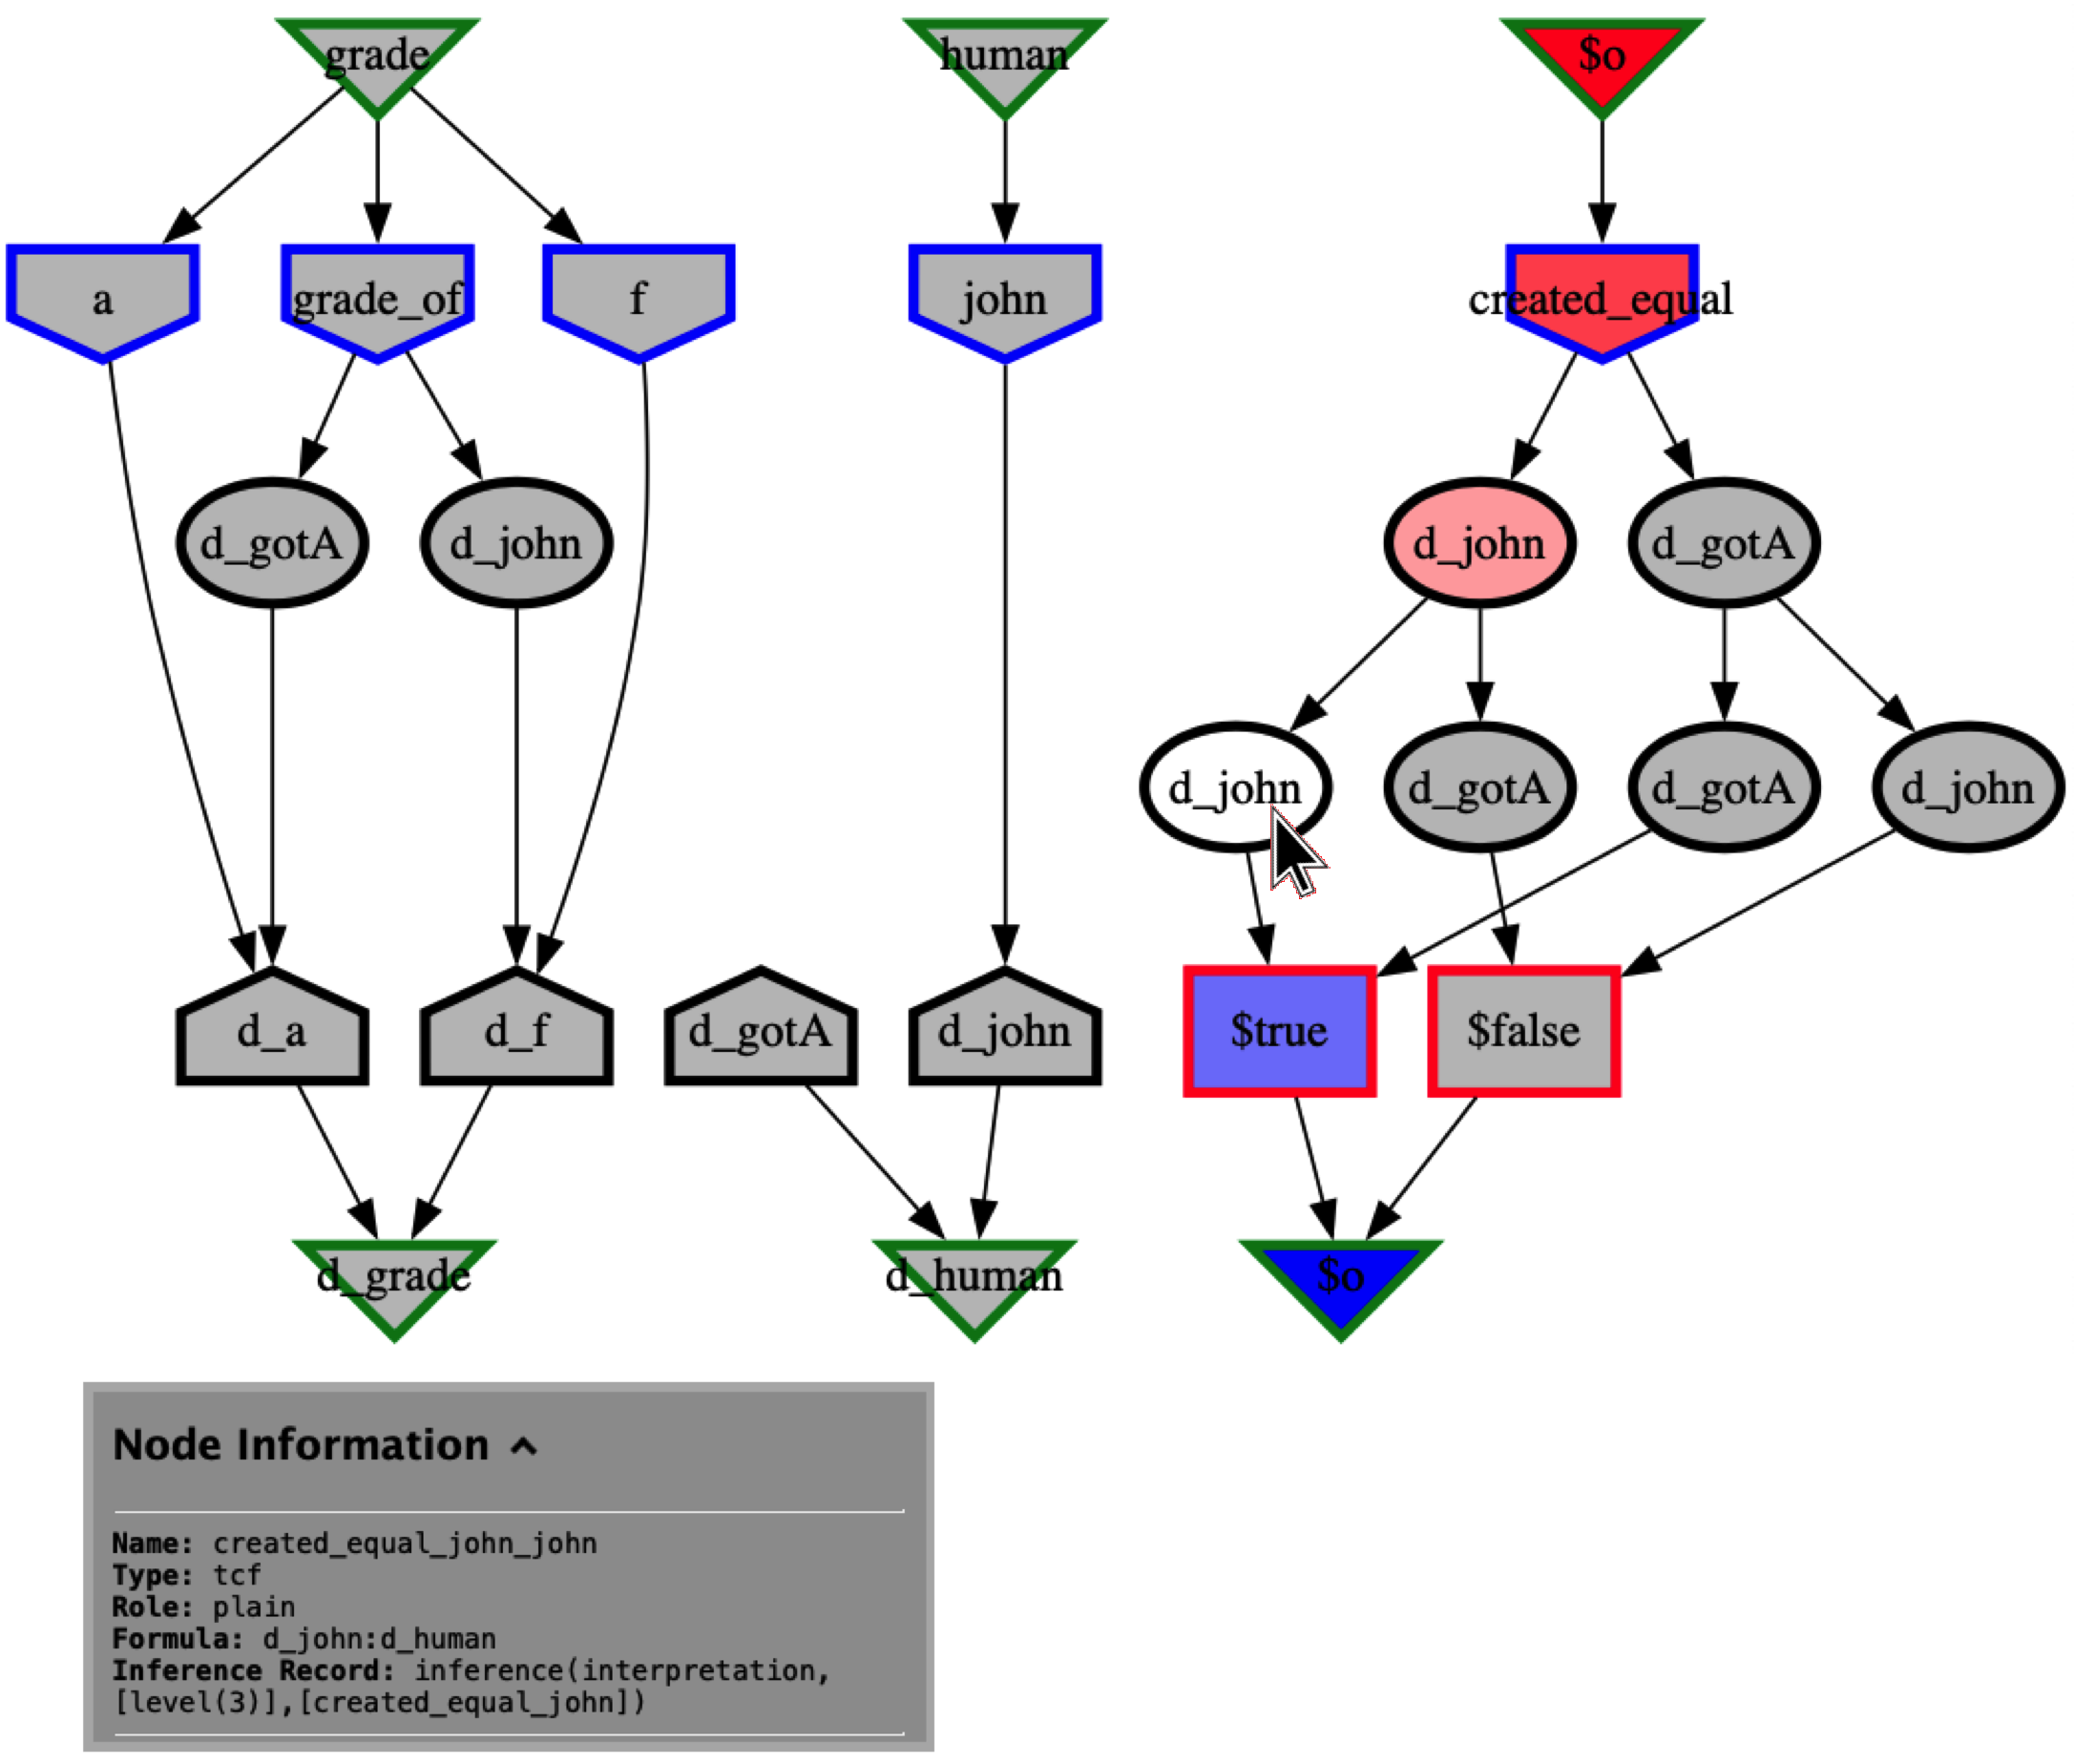
\includegraphics[width=\columnwidth]{TFF_Finite.s.IIV.pdf}
\caption{Visualization of the interpretation in Figure~\ref{TF0FiniteInterpretation}}
\label{TF0FiniteIIV}
\end{figure}

Figure~\ref{TF0InfiniteIIV} is the visualization of the infinite model in 
Figure~\ref{TF0InfiniteInterpretation}. 
Here (universally quantified) variables are used to represent the infinite number of
domain elements, and builtin arithmetic predicates used to compute the symbols' mappings.
Here the cursor is hovering over the {\smalltt{X:\$int}} node, showing how 
{\smalltt{child\_of(X)}} is interpreted as {\smalltt{\$sum(X,1)}}.
This interactive visualization is available in the IIV tool using 
{\scriptsize {\tt https://raw.githubusercontent.com/ GeoffsPapers/ModelVerification/main/TFF\_Integer.s.IIV}}
as the ``URL to fetch from''.

\begin{figure}[htbp]
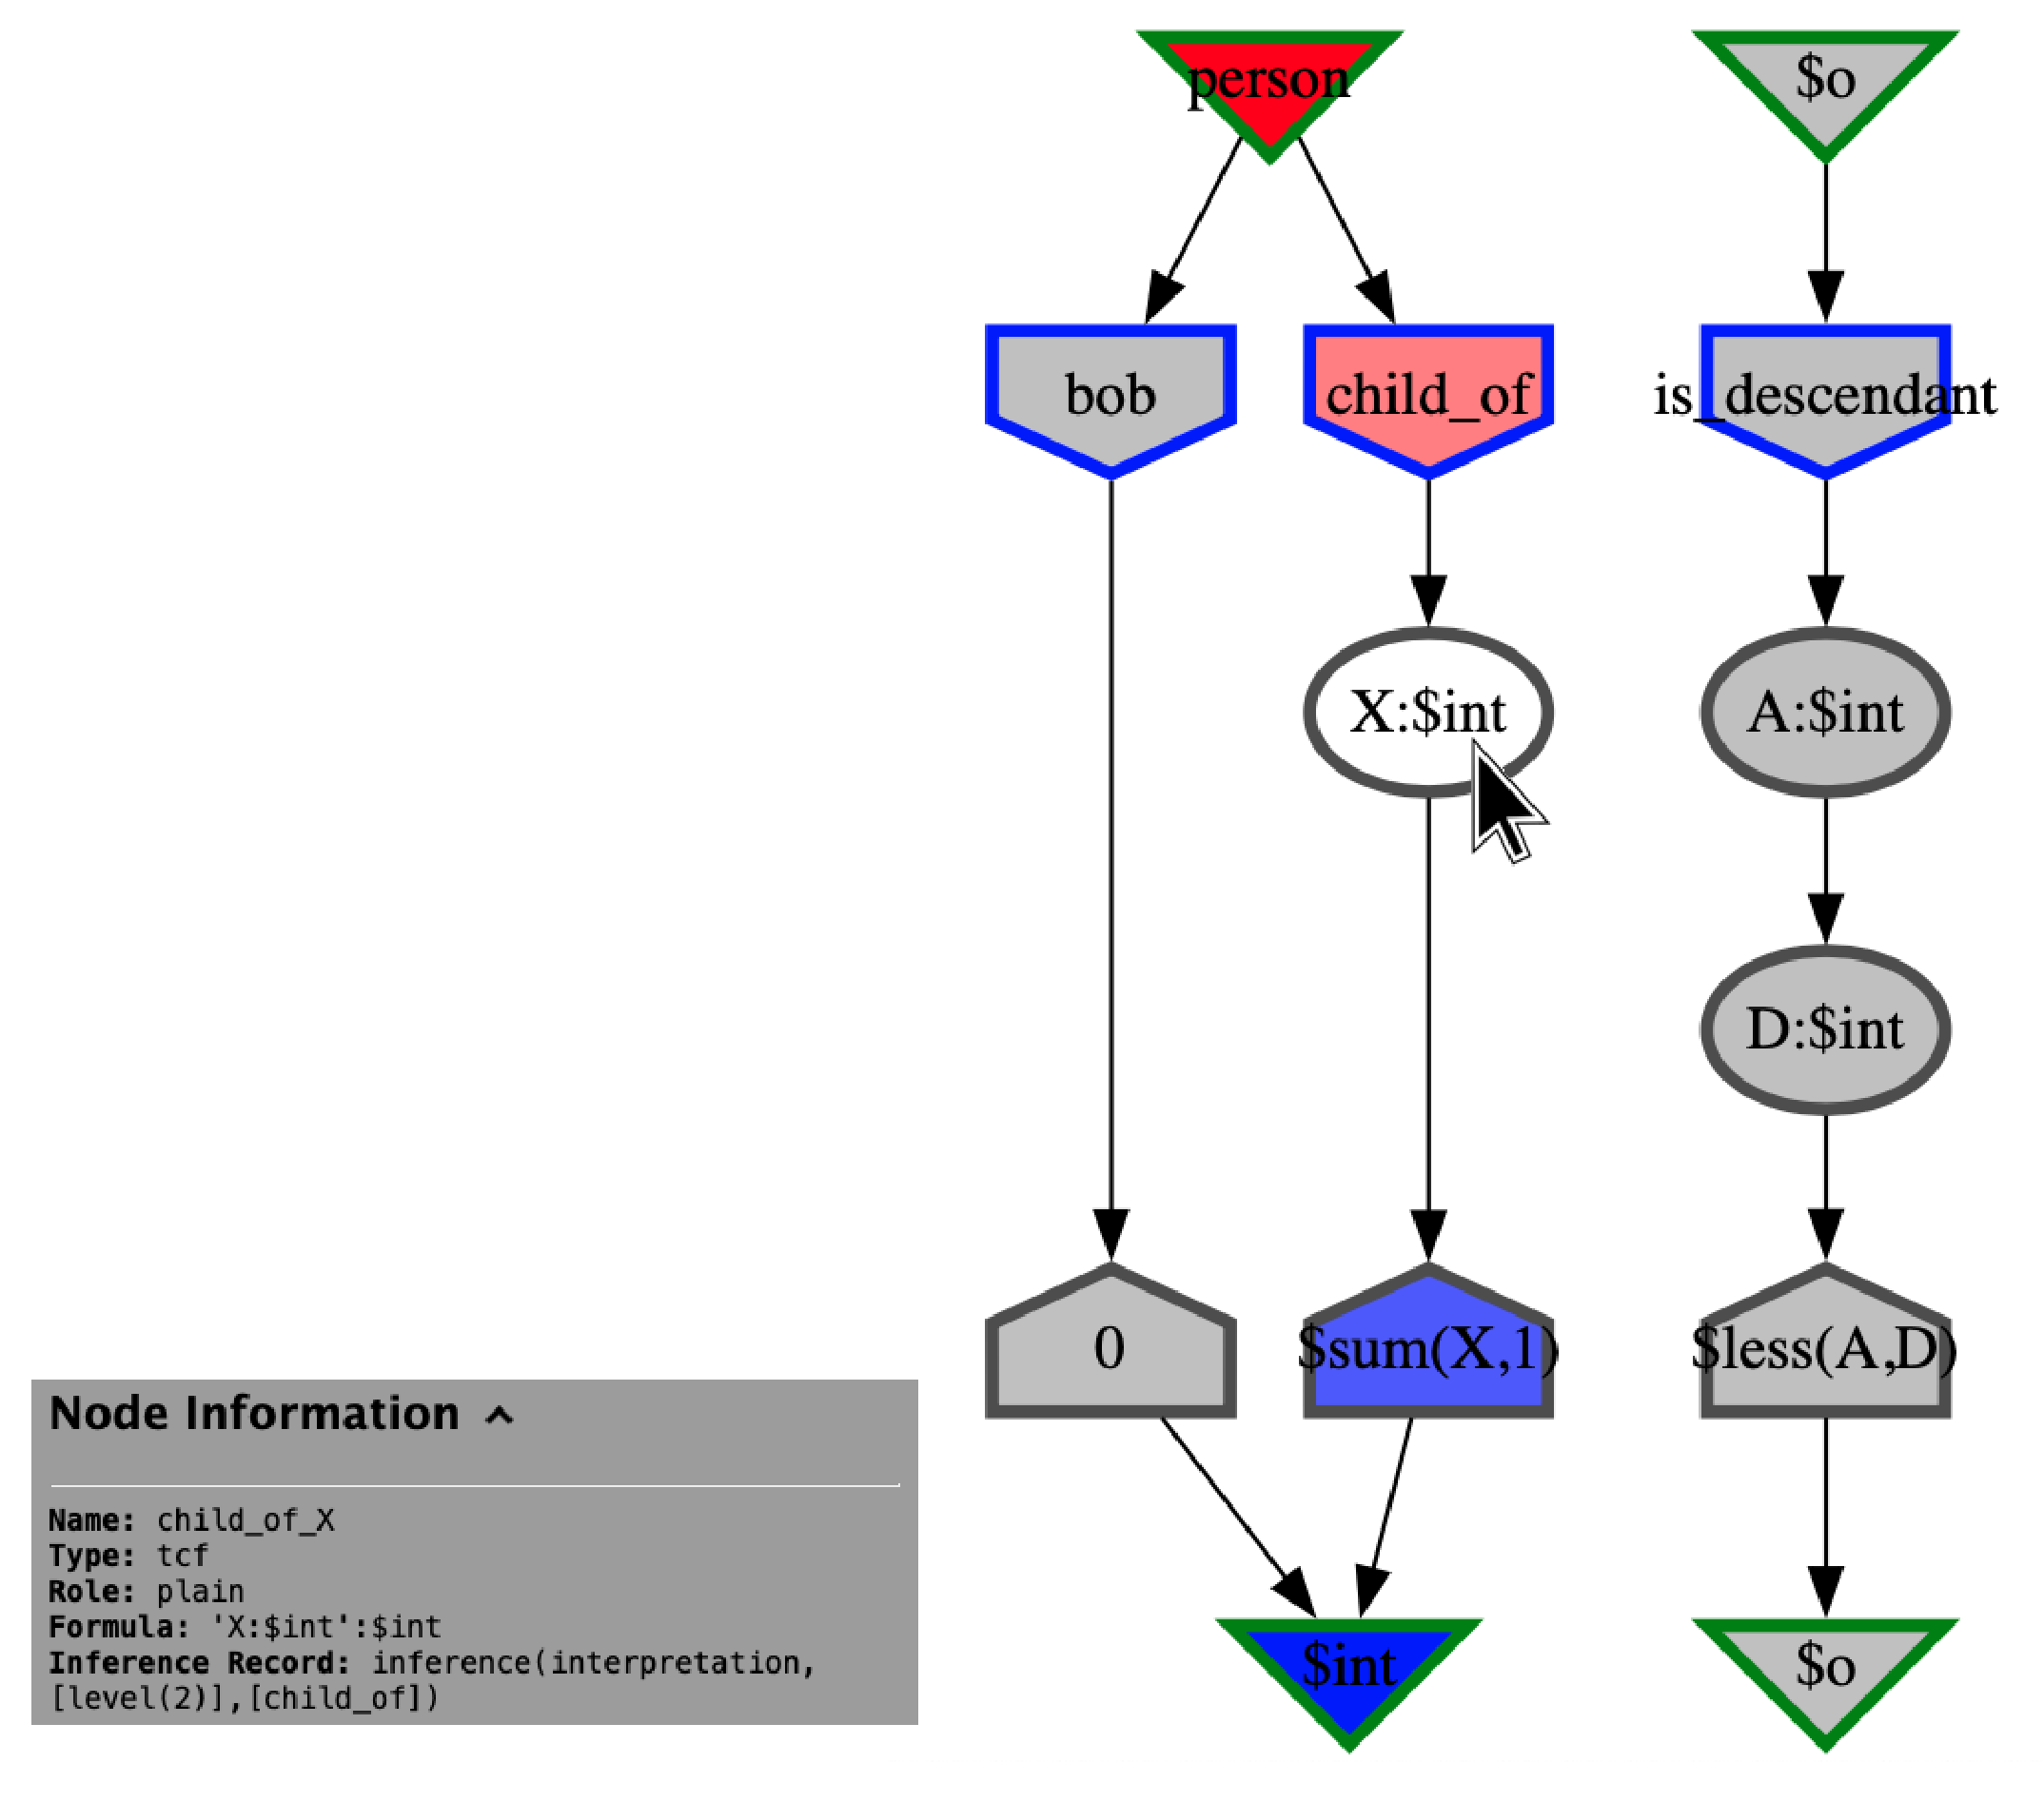
\includegraphics[width=\columnwidth]{TFF_Integer.s.IIV.pdf}
\caption{Visualization of the interpretation in Figure~\ref{TF0InfiniteInterpretation}}
\label{TF0InfiniteIIV}
\end{figure}

At this stage the implementation is prototype in the sense that an interpretation formula
has to be manually translated into the input format for IIV.
Further inspiration might lead to improvements to these visualizations, especially for more
complex infinite interpretations.

%--------------------------------------------------------------------------------------------------
\section{Conclusion}
\label{Conclusion}

%--------------------------------------------------------------------------------------------------
\bibliographystyle{flairs}
\bibliography{Bibliography.bib}
%--------------------------------------------------------------------------------------------------
\end{document}
%--------------------------------------------------------------------------------------------------
%% \section{Formatting Requirements in Brief}
%% We need source and PDF files that can be used in a variety of ways and can be output on a variety of devices. FLAIRS imposes some requirements on your source and PDF files that must be followed. Most of these requirements are based on our efforts to standardize conference manuscript properties and layout. These requirements are as follows, and all papers submitted to FLAIRS for publication must comply:
%% 
%% \begin{itemize}
%% \item Your .tex file must compile in PDF\LaTeX{} --- \textbf{ no .ps or .eps figure files.}
%% \item All fonts must be embedded in the PDF file --- \textbf{ this includes your figures.}
%% \item Modifications to the style sheet (or your document) in an effort to avoid extra page  are NOT allowed.
%% \item No type 3 fonts may be used (even in illustrations).
%% \item Your title must follow US capitalization rules.
%% \item \LaTeX{} documents must use the Times or Nimbus font package (do not use Computer Modern for the text of your paper).
%% \item Fonts that require non-English language support (CID and Identity-H) must be converted to outlines or removed from the document (even if they are in a graphics file embedded in the document). 
%% \item Two-column format is required for all papers.
%% \item The paper size for final submission must be US letter. No exceptions.
%% \item The source file must exactly match the PDF.
%% \item The document margins must be as specified in the formatting instructions.
%% \item The number of pages and the file size must be as specified for your event.
%% \item No document may be password protected.
%% \item Neither the PDFs nor the source may contain any embedded links or bookmarks.
%% \item Your source and PDF must not have any page numbers, footers, or headers.
%% \item Your PDF must be compatible with Acrobat 5 or higher.
%% \item Your \LaTeX{} source file (excluding references) must consist of a \textbf{single} file (use of the ``input" command is not allowed.
%% \item Your graphics must be sized appropriately outside of \LaTeX{} (do not use the ``clip" command) .
%% \end{itemize}
%% 
%% If you do not follow the above requirements, it is likely that we will be unable to publish your paper.
%% 
%% \section{What Files to Submit}
%% You must submit the following items to ensure that your paper is published:
%% \begin{itemize}
%% \item A fully-compliant PDF file.
%% \item Your  \LaTeX{}  source file submitted as a \textbf{single} .tex file (do not use the ``input" command to include sections of your paper --- every section must be in the single source file). The only exception is the bibliography, which you may include separately. Your source must compile on our system, which includes the standard \LaTeX{} support files.
%% \item All your graphics files.
%% \item The \LaTeX{}-generated files (e.g. .aux and .bib file, etc.) for your compiled source.
%% \item All the nonstandard style files (ones not commonly found in standard \LaTeX{} installations) used in your document (including, for example, old algorithm style files). If in doubt, include it.
%% \end{itemize}
%% 
%% Your \LaTeX{} source will be reviewed and recompiled on our system (if it does not compile, you may incur late fees).   \textbf{Do not submit your source in multiple text files.} Your single \LaTeX{} source file must include all your text, your bibliography (formatted using flairs.bst), and any custom macros. Accompanying this source file, you must also supply any nonstandard (or older) referenced style files and all your referenced graphics files. 
%% 
%% Your files should work without any supporting files (other than the program itself) on any computer with a standard \LaTeX{} distribution. Place your PDF and source files in a single tar, zipped, gzipped, stuffed, or compressed archive. Name your source file with your last (family) name.
%% 
%% \textbf{Do not send files that are not actually used in the paper.} We don't want you to send us any files not needed for compiling your paper, including, for example, this instructions file, unused graphics files, and so forth.  
%% 
%% \section{Using \LaTeX{} to Format Your Paper}
%% 
%% The latest version of the FLAIRS style file is available on FLAIRS's website. Download this file and place it in a file named ``flairs.sty" in the \TeX\ search path. Placing it in the same directory as the paper should also work. You must download the latest version.
%% 
%% The following packages are incompatible with flairs.sty and/or flairs.bst and must not be used (this list is not exhaustive --- there are others as well):
%% \begin{itemize}
%% \item hyperref
%% \item natbib
%% \item geometry
%% \item titlesec
%% \item layout
%% \item caption
%% \item titlesec
%% \item T1 fontenc package (install the CM super fonts package instead)
%% \end{itemize}
%% 
%% \subsection{Illegal Commands}
%% The following commands may not be used in your paper:
%% \begin{itemize}
%% \item \textbackslash input
%% \item \textbackslash vspace (when used before or after a section or subsection)
%% \item \textbackslash addtolength 
%% \item \textbackslash columnsep
%% \item \textbackslash top margin (or text height or addsidemargin or even side margin)
%% \end{itemize}
%% 
%% \subsection{Paper Size, Margins, and Column Width}
%% Papers must be formatted to print in two-column format on 8.5 x 11 inch US letter-sized paper. The margins must be exactly as follows: 
%% \begin{itemize}
%% \item Top margin: .75 inches
%% \item Left margin: .75 inches
%% \item Right margin: .75 inches
%% \item Bottom margin: 1.25 inches
%% \end{itemize} 
%% 
%% 
%% The default paper size in most installations of \LaTeX{} is A4. However, because we require that your electronic paper be formatted in US letter size, you will need to alter the default for this paper to US letter size. Assuming you are using the 2e version of \LaTeX{}, you can do this by including the [letterpaper] option at the beginning of your file: 
%% \textbackslash documentclass[letterpaper]{article}. 
%% 
%% This command is usually sufficient to change the format. Sometimes, however, it may not work. Use PDF\LaTeX{} and include
%% \textbackslash setlength\{\textbackslash pdfpagewidth\}\{8.5in\}
%% \textbackslash setlength\{\textbackslash pdfpageheight\}\{11in\}
%% in your preamble. 
%% 
%% \textbf{Do not use the Geometry package to alter the page size.} Use of this style file alters flairs.sty and will result in your paper being rejected. 
%% 
%% 
%% \subsubsection{Column Width and Margins.}
%% To ensure maximum readability, your paper must include two columns. Each column should be 3.3 inches wide (slightly more than 3.25 inches), with a .375 inch (.952 cm) gutter of white space between the two columns. The flairs.sty file will automatically create these columns for you. 
%% 
%% \subsection{Overlength Papers}
%% If your paper is too long, turn on \textbackslash frenchspacing, which will reduce the space after periods. Next,  shrink the size of your graphics. Use \textbackslash centering instead of \textbackslash begin\{center\} in your figure environment. If these two methods don't work, you may minimally use the following. For floats (tables and figures), you may minimally reduce \textbackslash floatsep, \textbackslash textfloatsep, \textbackslash abovecaptionskip, and \textbackslash belowcaptionskip. For mathematical environments, you may minimally reduce \textbackslash abovedisplayskip, \textbackslash belowdisplayskip, and \textbackslash arraycolsep. You may also alter the size of your bibliography by inserting \textbackslash fontsize\{9.5pt\}\{10.5pt\} \textbackslash selectfont
%% right before the bibliography. 
%% 
%% Commands that alter page layout are forbidden. These include \textbackslash columnsep, \textbackslash topmargin, \textbackslash topskip, \textbackslash textheight, \textbackslash textwidth, \textbackslash oddsidemargin, and \textbackslash evensizemargin (this list is not exhaustive). If you alter page layout, you will be required to pay the page fee \textit{plus} a reformatting fee. Other commands that are questionable and may cause your paper to be rejected include  \textbackslash parindent, and \textbackslash parskip. Commands that alter the space between sections are also questionable. The title sec package is not allowed. Regardless of the above, if your paper is obviously ``squeezed" it is not going to to be accepted. Before using every trick you know to make your paper a certain length, try reducing the size of your graphics or cutting text instead.
%% 
%% \subsection{Credits}
%% Any credits to a sponsoring agency should appear in the acknowledgments section, unless the agency requires different placement. If it is necessary to include this information on the front page, use
%% \textbackslash thanks in either the \textbackslash author or \textbackslash title commands.
%% For example:
%% \begin{quote}
%% \begin{small}
%% \textbackslash title\{Very Important Results in AI\textbackslash thanks\{This work is
%%  supported by everybody.\}\}
%% \end{small}
%% \end{quote}
%% Multiple \textbackslash thanks commands can be given. Each will result in a separate footnote indication in the author or title with the corresponding text at the botton of the first column of the document. Note that the \textbackslash thanks command is fragile. You will need to use \textbackslash protect.
%% 
%% Please do not include \textbackslash pubnote commands in your document.
%% 
